\chapter{Pré-processamento de Dados}
\label{chap:preprocessamento_de_dados}

\section{Preparação dos Dados}

Os dados utilizados neste estudo foram coletados em sessões experimentais com atletas profissionais de basquetebol feminino, submetidas a condições de estimulação transcraniana por corrente contínua de alta definição (HD-tDCS) e a uma condição de controle (sham). Neste capítulo, descrevemos os procedimentos realizados para organizar, sincronizar e preparar os sinais de eletroencefalografia (EEG) e eletrocardiografia (ECG) para análise.

\subsection{Organização Inicial dos Dados}

Os dados de EEG e ECG foram armazenados em arquivos separados, correspondentes a cada atleta e condição experimental (\textit{pre\_sham}, \textit{post\_sham}, \textit{pre\_cathodic}, \textit{post\_cathodic}). Os sinais de EEG foram originalmente registrados a 1000 Hz, enquanto os sinais de ECG – obtidos a partir do EMG do músculo peitoral maior – foram registrados a 1111,11 Hz. Nesta etapa, os arquivos foram:
\begin{itemize}
    \item Identificados e associados a cada atleta e condição;
    \item Renomeados e normalizados para garantir consistência;
    \item Submetidos a uma verificação de integridade para evitar erros no processamento.
\end{itemize}

\subsection{Sincronização Temporal entre EEG e ECG}

Devido ao início não sincronizado das gravações, foi necessário alinhar temporalmente os sinais de EEG e ECG. Com base em marcadores do período baseline, os seguintes passos foram realizados:
\begin{itemize}
    \item Extração dos tempos de início e fim do baseline para cada modalidade;
    \item Remoção dos primeiros e últimos 15 segundos de cada gravação, minimizando artefatos de borda;
    \item Ajuste dos timestamps para que os sinais iniciassem simultaneamente;
\end{itemize}

\subsection{Estruturação dos Dados}

Após a sincronização, os dados foram organizados para o processamento subsequente. Os sinais de EEG foram armazenados em formato FIF, preservando as informações dos canais e os metadados, enquanto os dados de ECG foram exportados em formato CSV.


\section{Pré-processamento dos Sinais}

Esta seção descreve os procedimentos aplicados para garantir a qualidade dos sinais, incluindo filtragem, remoção de artefatos e segmentação.

\subsection{Pré-processamento do EEG}

\subsubsection{Filtragem, Reamostragem e Preparação dos Dados de EEG}

O processamento dos dados de EEG envolveu as seguintes etapas:
\begin{itemize}
    \item \textbf{Aquisição e Carregamento:} Os dados brutos foram baixados do Google Drive e carregados via MNE-Python a partir de arquivos exportados do software BrainVision (ou, alternativamente, em formato EEGLAB). Após o carregamento, os canais foram renomeados conforme uma convenção padronizada (por exemplo, Fp1, Fz, F3, etc.) e canais irrelevantes foram removidos. (Ver Figura~\ref{fig:exemplo_sinais_eeg})
    \item \textbf{Aplicação de Montage:} Foi aplicado o montage padrão \textit{standard\_1005} para assegurar a correta localização dos eletrodos, conforme ilustrado no diagrama do sistema 10-20. (Ver Figura~\ref{fig:sistema_10_20})
    \item \textbf{Definição do Período de Análise:} Com base nas informações extraídas dos arquivos de baseline, os dados foram recortados para um intervalo que excluiu os primeiros e últimos 15 segundos da gravação, reduzindo artefatos de borda.
    \item \textbf{Filtragem:} Aplicou-se um filtro passa-banda entre 0,5 e 60 Hz para eliminar ruídos fora do intervalo de interesse, seguido de um filtro notch em 60 Hz para remover interferências da rede elétrica.
    \item \textbf{Reamostragem:} Para padronizar a taxa de amostragem e facilitar o alinhamento com outros sinais (como o ECG), os dados de EEG foram reamostrados para 500 Hz.
\end{itemize}

\begin{figure}[htb]
    \centering
    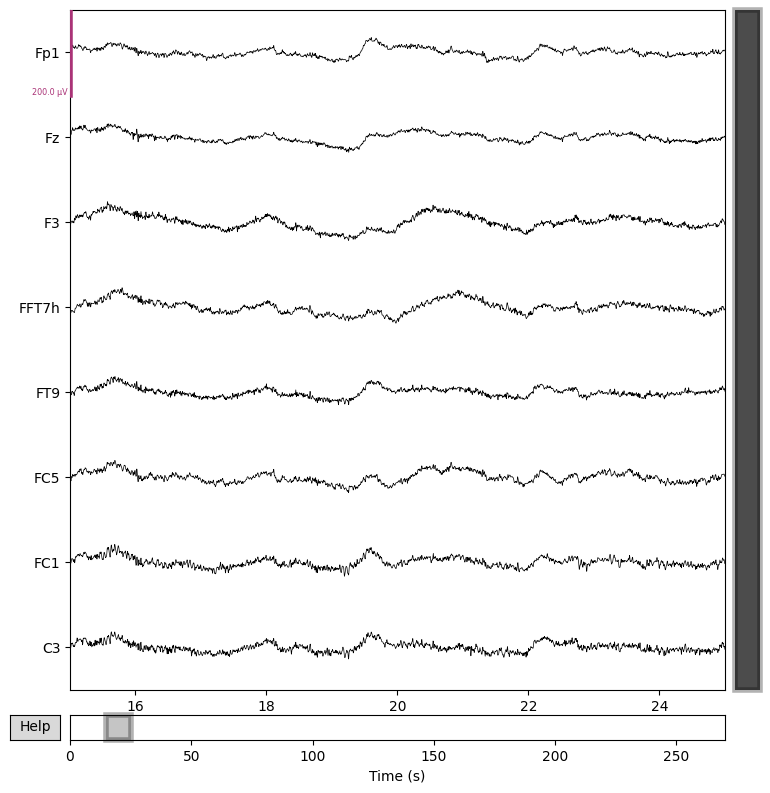
\includegraphics[width=0.8\textwidth]{figs/1_preprocessamento_eeg/2_exemplo_sinais_canais_eeg.png}
    \caption{Exemplo de sinais brutos de EEG, ilustrando a variação natural dos canais ao longo do tempo.}
    \label{fig:exemplo_sinais_eeg}
\end{figure}

\begin{figure}[htb]
    \centering
    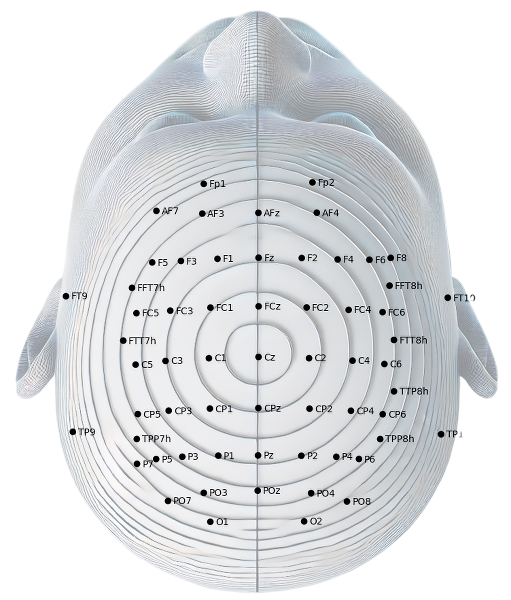
\includegraphics[width=0.8\textwidth]{figs/1_preprocessamento_eeg/1_sistema_10_20.png}
    \caption{Diagrama do sistema 10-20, demonstrando a localização padronizada dos eletrodos no couro cabeludo.}
    \label{fig:sistema_10_20}
\end{figure}

\subsubsection{Limpeza de Artefatos e Remoção de Componentes de Ruído (ICA)}

Para aprimorar a qualidade dos sinais de EEG, foi empregada a Análise de Componentes Independentes (ICA) conforme as seguintes etapas:
\begin{itemize}
    \item \textbf{Definição dos Componentes:} O número de componentes foi definido igual ao número de canais bons disponíveis (excluindo os canais previamente identificados como ruins por inspeção visual).
    \item \textbf{Aplicação do ICA:} Utilizou-se o método FastICA para decompor o sinal, preservando as informações críticas para a análise de sincronicidade.
    \item \textbf{Estimativa de Parâmetros de Rejeição:} A biblioteca \textit{autoreject} foi empregada para determinar, através de épocas de duração fixa, os limites ideais para rejeição de artefatos.
    \item \textbf{Identificação Automática de Artefatos:} Componentes relacionados a artefatos oculares (usando canais como Fp1 e Fp2) e à atividade cardíaca foram identificados automaticamente. Adicionalmente, uma análise baseada na curtose foi realizada para detectar componentes com alta amplitude, indicativos de artefatos.
    \item \textbf{Inspeção Visual e Seleção:} Foram gerados gráficos das propriedades dos componentes e uma visualização interativa, inclusive com animação GIF, que permitiram a inspeção manual dos componentes para decidir quais excluir. (Ver Figuras~\ref{fig:componentes_pos_ICA})
    \item \textbf{Aplicação e Salvamento:} Após a definição dos componentes a serem removidos, o ICA foi aplicado para eliminar os artefatos identificados, gerando um sinal de EEG limpo, que foi salvo em formato FIF para futuras análises.
\end{itemize}

\begin{figure}[htb]
    \centering
    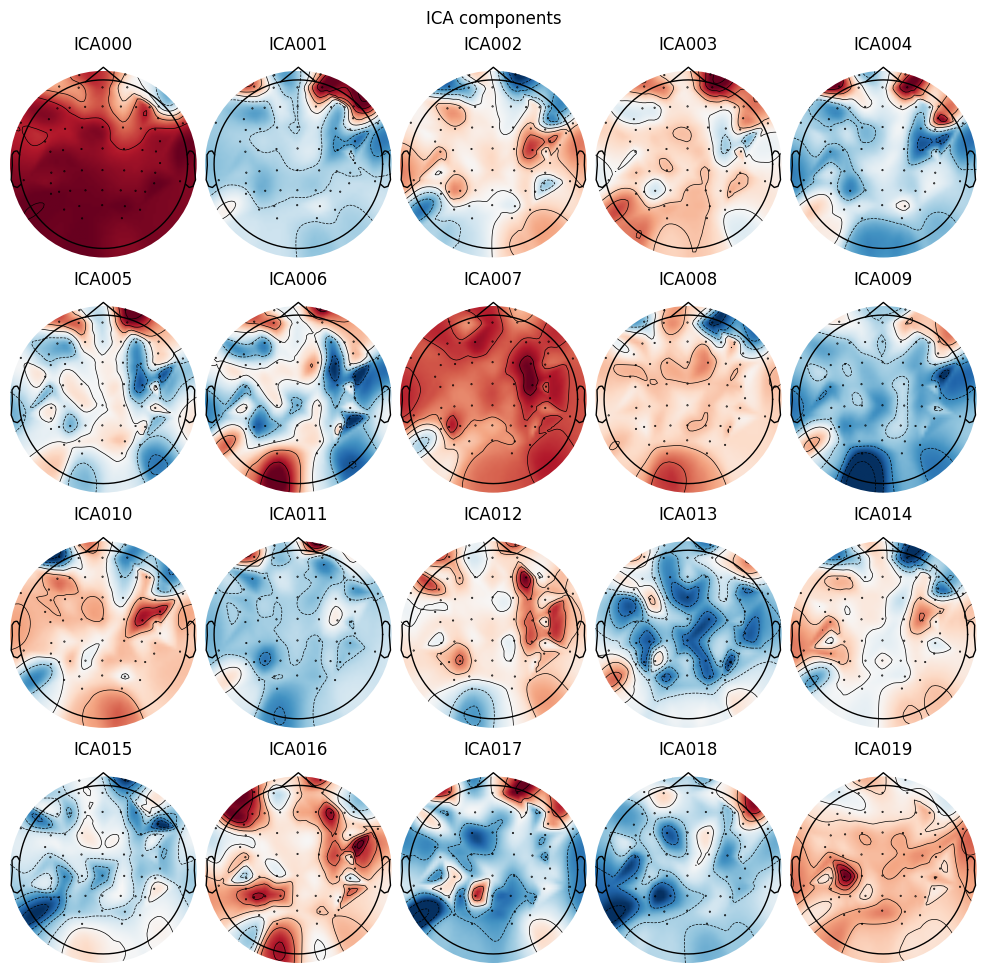
\includegraphics[width=0.8\textwidth]{figs/1_preprocessamento_eeg/3_exemplo_compomentes_pos_ICA.png}
    \caption{Exemplo de componentes obtidos após a aplicação do ICA, com mapas topográficos que evidenciam a distribuição espacial de cada componente.}
    \label{fig:componentes_pos_ICA}
\end{figure}

\begin{figure}[htb]
    \centering
    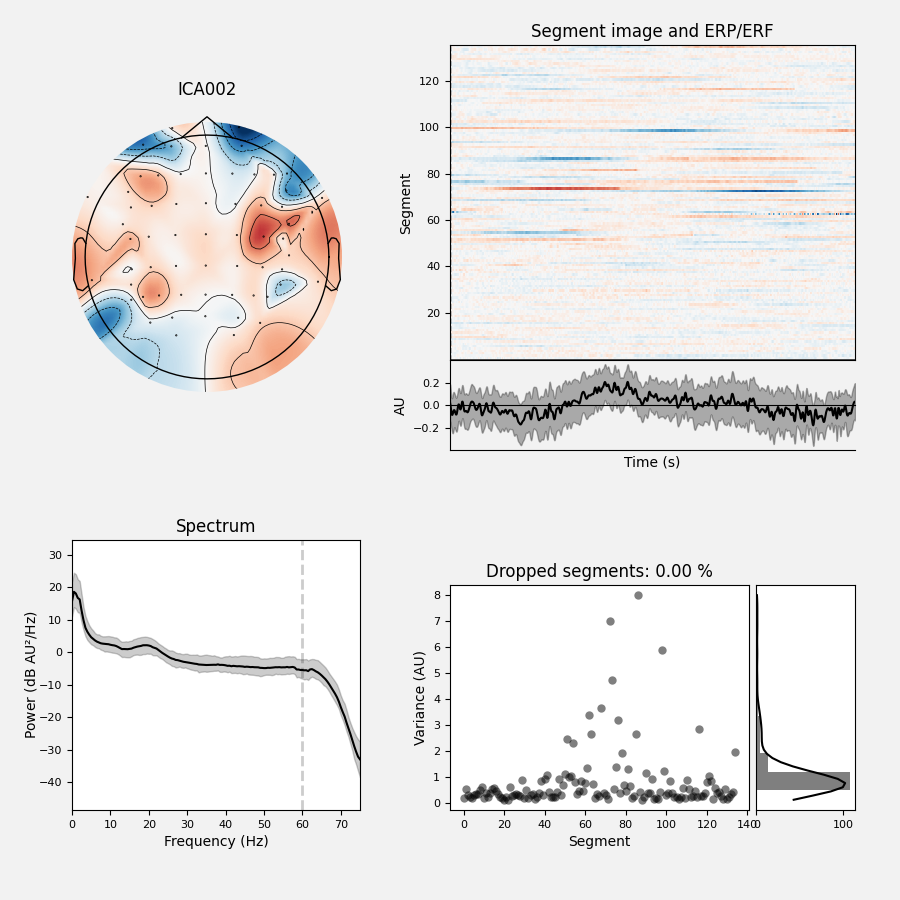
\includegraphics[width=0.8\textwidth]{figs/1_preprocessamento_eeg/4_exemplo_ICA_component_analysis.png}
    \caption{Exemplo de análise detalhada de um componente ICA, apresentando o mapa topográfico, o espectro de frequência e outras características relevantes para a identificação de artefatos.}
    \label{fig:exemplo_ICA_component_analysis}
\end{figure}


\subsection{Pré-processamento do Sinal de ECG}
\label{subsec:preprocess_ecg}

O processamento do sinal de ECG foi realizado com o objetivo de obter uma versão limpa e refinada do sinal, que permitisse a detecção precisa dos R-peaks e a extração de informações de fase. As etapas foram organizadas da seguinte forma:

\subsubsection{Aquisição e Segmentação dos Dados de ECG}

\begin{itemize}
    \item \textbf{Aquisição:} Os dados de ECG foram coletados juntamente com informações sobre os tempos de início e fim do período de baseline para cada condição experimental, garantindo a correta identificação dos intervalos de interesse para análise.
    \item \textbf{Segmentação:} Com base nos tempos extraídos dos arquivos de baseline, o sinal bruto foi segmentado para selecionar apenas o intervalo correspondente à condição de interesse. Para reduzir artefatos nas bordas, os primeiros e últimos 15 segundos foram removidos.
\end{itemize}

\subsubsection{Limpeza do Sinal e Detecção de Picos}

\begin{itemize}
    \item \textbf{Limpeza:} Utilizou-se a biblioteca NeuroKit2 para processar o sinal segmentado e remover ruídos, gerando uma versão limpa do ECG.
    
    \item \textbf{Detecção Automática de Picos:} Foi aplicado um algoritmo para detecção automática dos picos R (R-peaks) no sinal limpo, identificando os batimentos cardíacos. A Figura~\ref{fig:ecg_picos_detectados} ilustra um exemplo em que o sinal bruto (cinza) é sobreposto ao sinal limpo (azul), enquanto os picos R são marcados em vermelho.
    
    \item \textbf{Correção Manual dos Picos R:} Após a detecção automática, foi realizada uma inspeção visual cuidadosa utilizando gráficos interativos para identificar:
    \begin{itemize}
        \item Ausência de picos em locais onde deveriam ocorrer, com inserção manual dos picos faltantes por meio da identificação precisa dos timestamps correspondentes.
        \item Presença de picos falsos em regiões sem batimentos válidos, com remoção manual desses picos com base nos timestamps detectados como incorretos.
    \end{itemize}
    Esse ajuste garante a acurácia na identificação dos batimentos cardíacos, evitando tanto a omissão quanto a inclusão indevida de eventos.
\end{itemize}

\begin{figure}[htb]
    \centering
    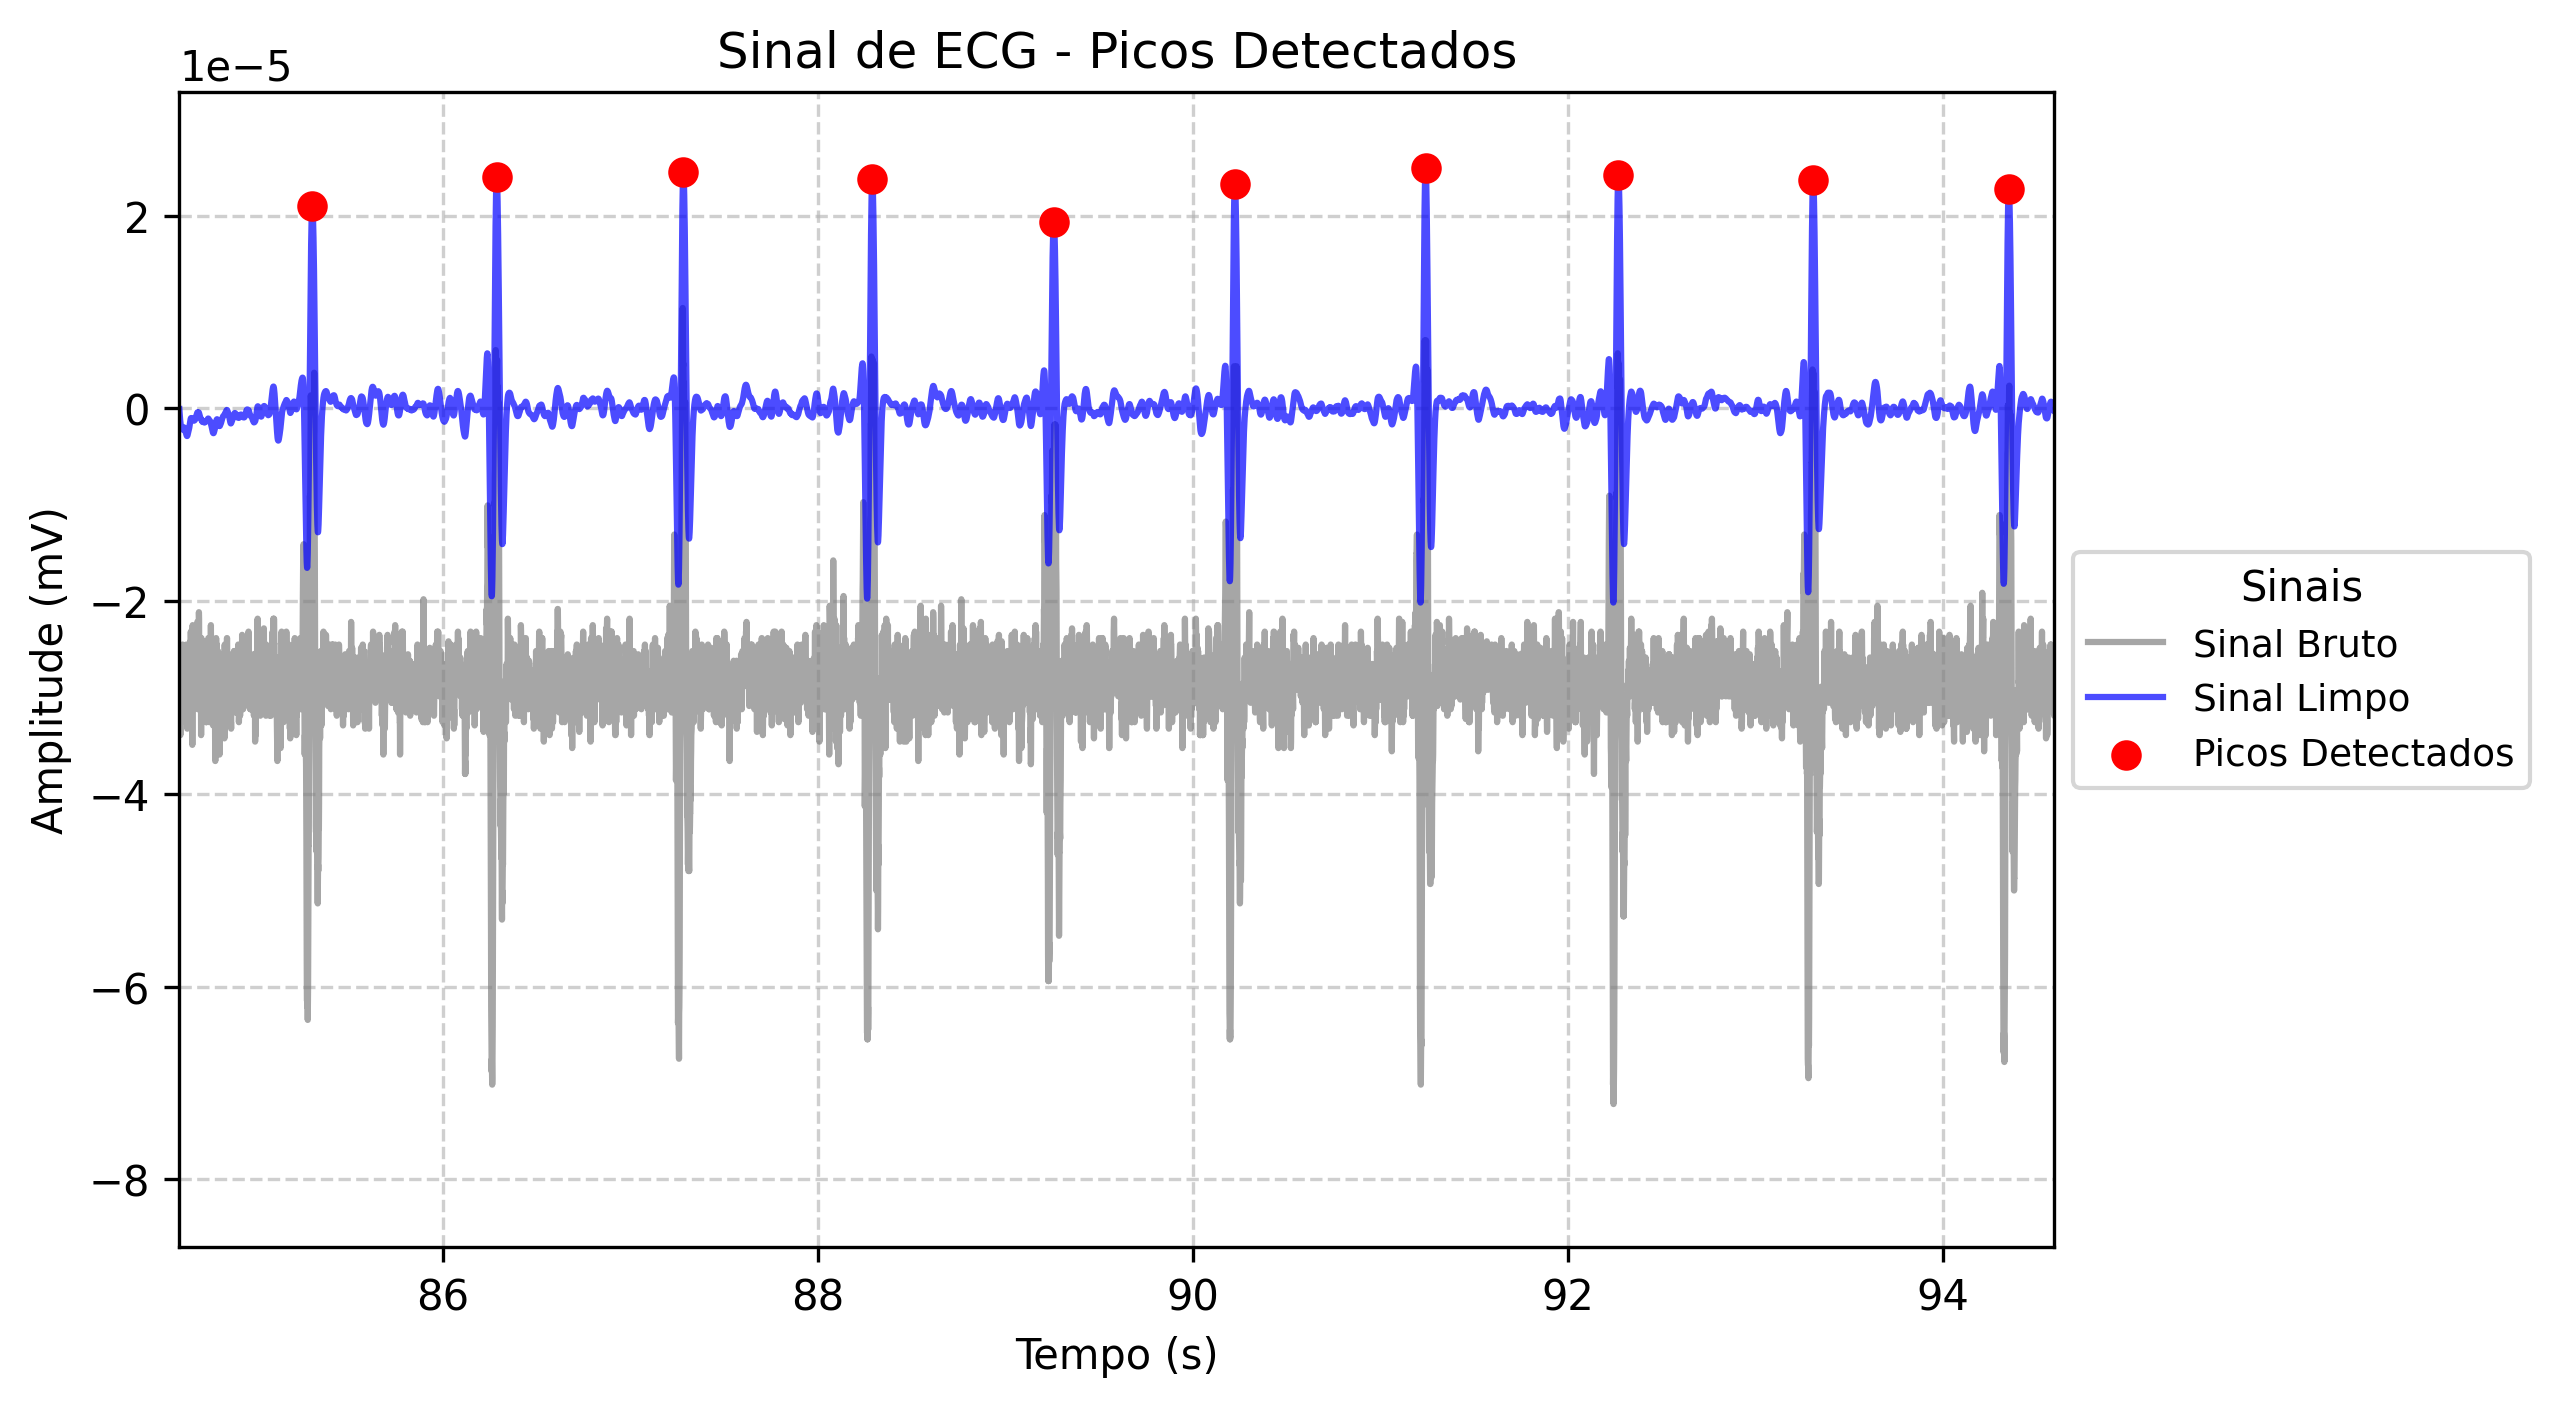
\includegraphics[width=0.8\textwidth]{figs/2_preprocessamento_ecg/1_Sinal_de_ECG_-_Picos_Detectados_zoom.png}
    \caption{Exemplo de sinal de ECG com picos detectados. O sinal bruto (cinza) é sobreposto pelo sinal limpo (azul), enquanto os picos R são marcados em vermelho.}
    \label{fig:ecg_picos_detectados}
\end{figure}

\subsubsection{Aplicação de Filtros Complementares}

Para refinar a definição dos eventos do ECG, foram aplicados filtros adicionais:
\begin{itemize}
    \item \textbf{Filtro de Janela:} Extração de uma janela de \(\pm50\) ms ao redor de cada pico, isolando os segmentos de interesse.
    \item \textbf{Filtro de Cruzamento pelo Zero:} Identificação dos pontos de cruzamento pelo zero nos segmentos próximos aos picos, para um ajuste fino dos limites dos eventos.
\end{itemize}
A combinação desses filtros resultou em um \emph{Sinal Final Filtrado}, que destaca de forma mais clara a morfologia do ECG. A Figura~\ref{fig:ecg_filtros_aplicados} exemplifica o efeito dos filtros, comparando o sinal limpo inicial (linha colorida) e o sinal final filtrado, bem como os picos detectados.

\begin{figure}[htb]
    \centering
    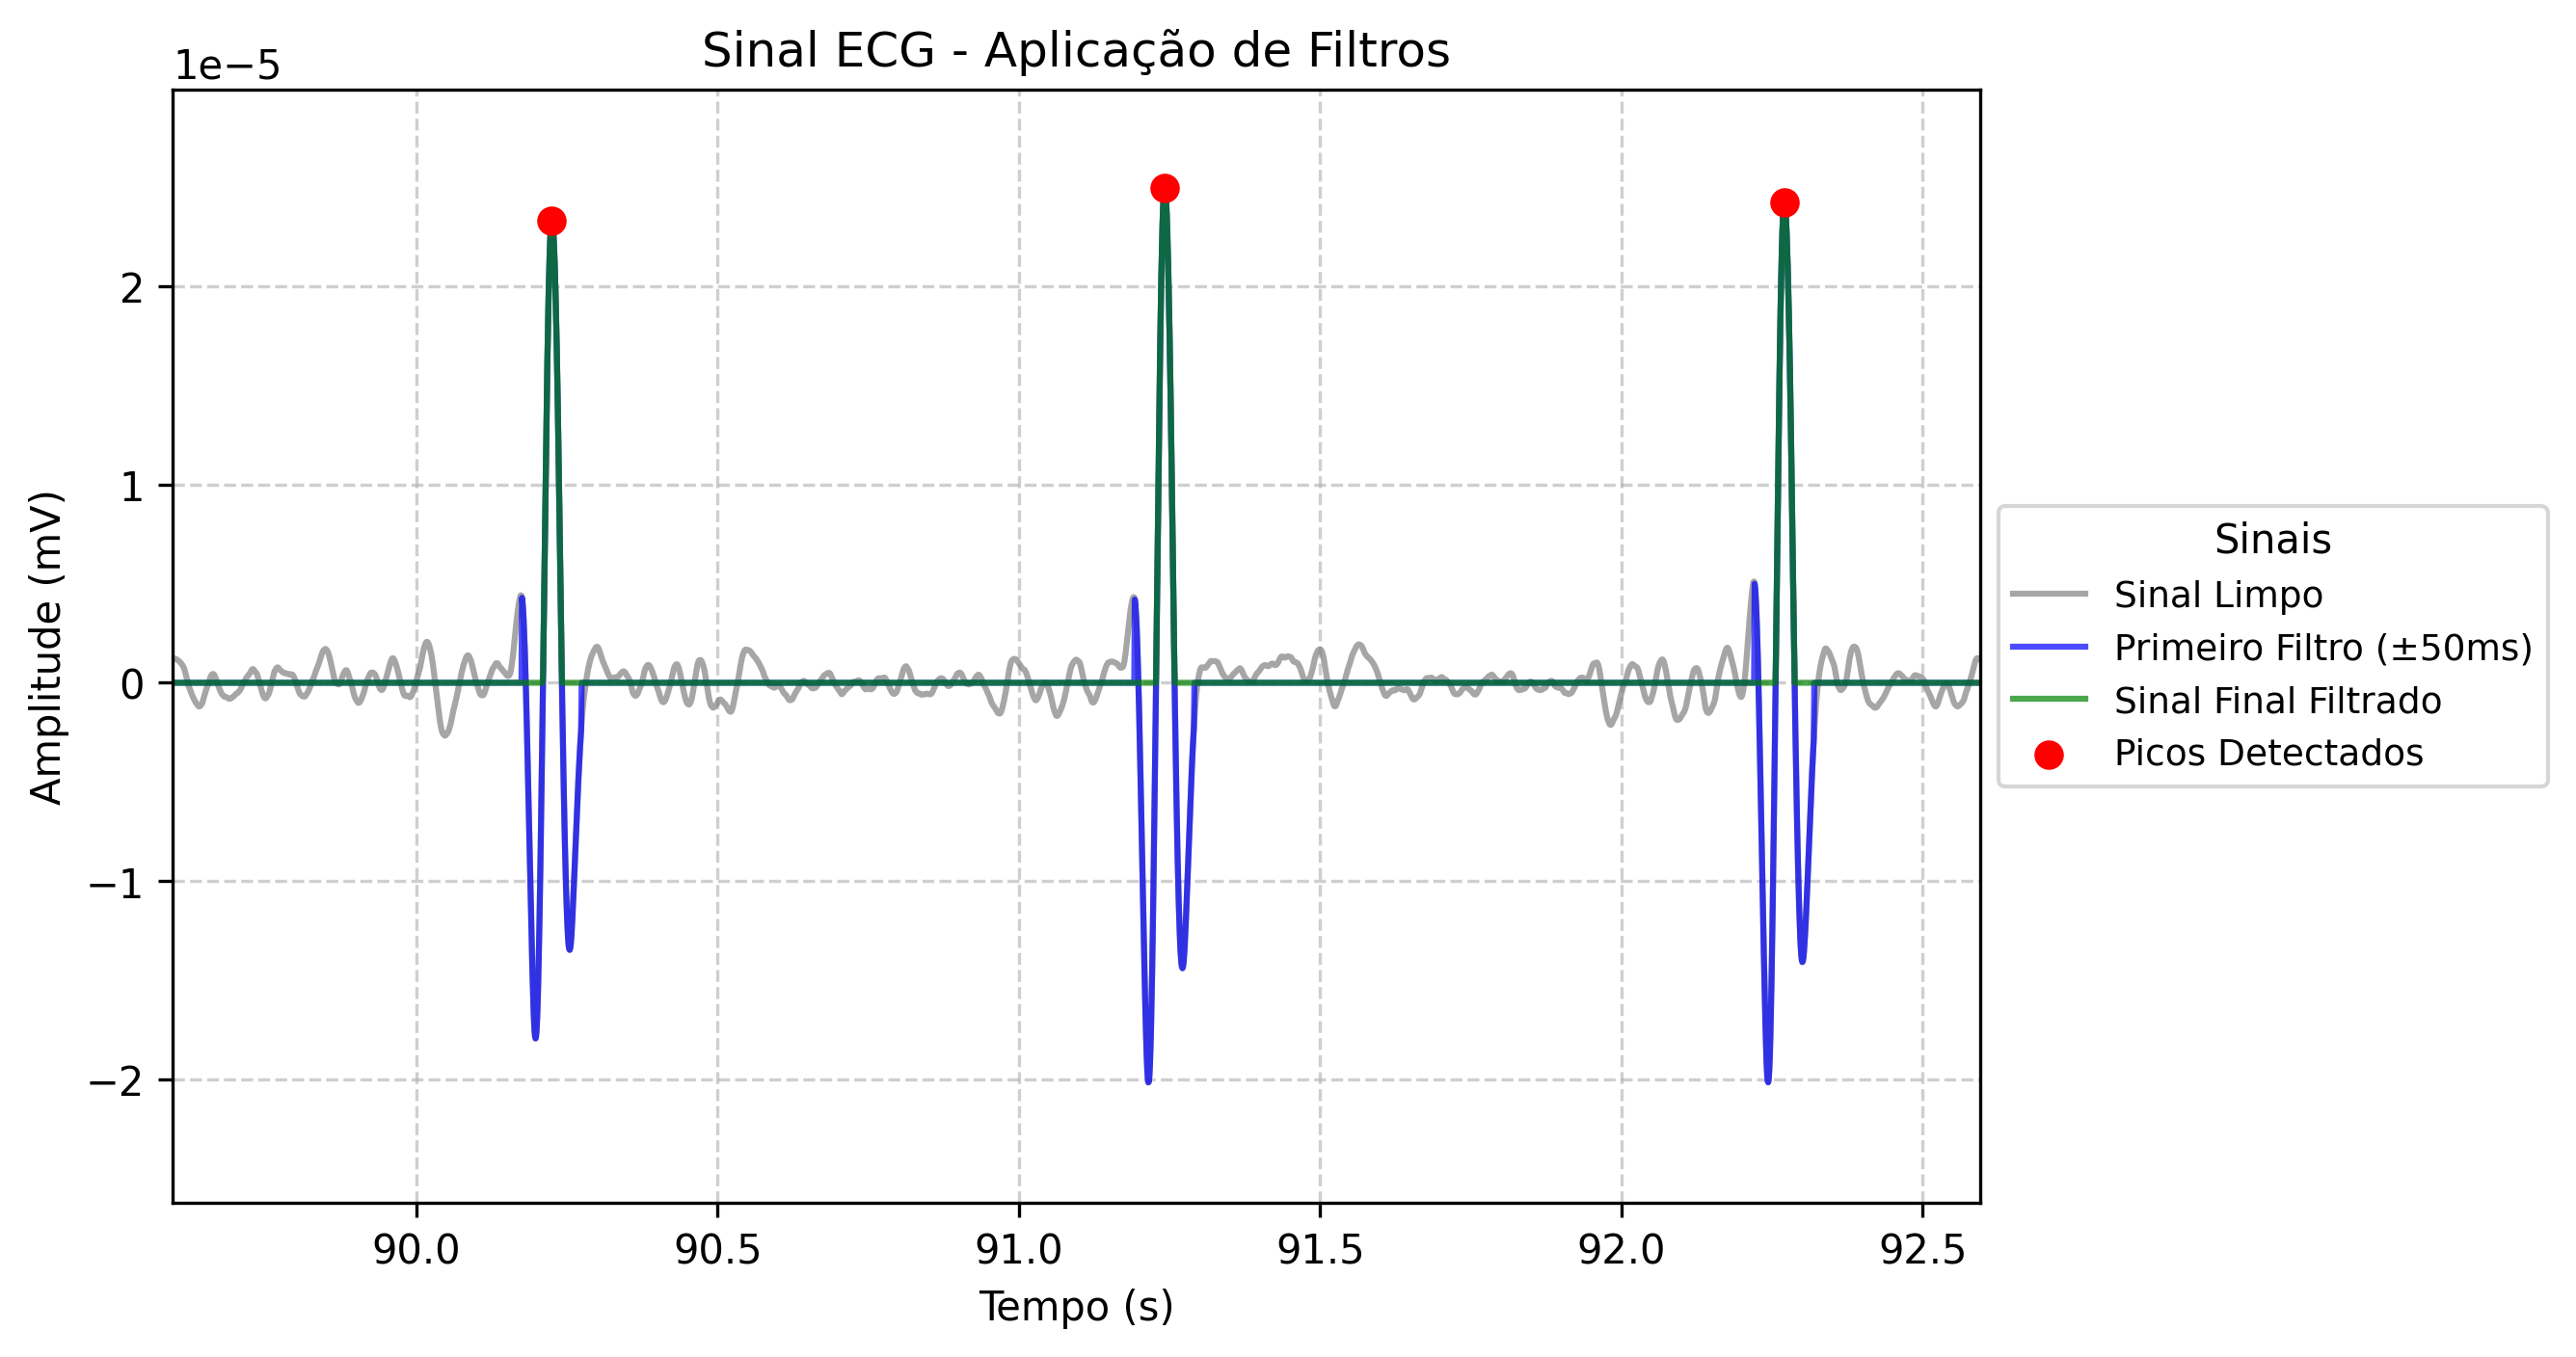
\includegraphics[width=0.8\textwidth]{figs/2_preprocessamento_ecg/2_Sinal_ECG_-_Aplicação_de_Filtros_zoom.png}
    \caption{Exemplo de aplicação de filtros complementares ao sinal de ECG, destacando a morfologia dos picos R (em vermelho).}
    \label{fig:ecg_filtros_aplicados}
\end{figure}

\subsubsection{Geração de Sinais Senoidais e Análise de Fase}

Para aprimorar a análise de sincronização de fase entre os sinais de EEG e ECG, o sinal de ECG foi transformado em uma representação senoidal. Essa transformação foi adotada pelos seguintes motivos:

\begin{itemize}
    \item \textbf{Definição Clara do Ciclo Cardíaco:} Ao utilizar os R-peaks para delimitar cada ciclo, a transformação em uma onda senoidal permite definir de forma inequívoca o início e o fim do ciclo cardíaco, proporcionando um marcador preciso para segmentar os períodos de interesse.
    \item \textbf{Extração Precisa da Fase:} Uma onda senoidal apresenta uma variação linear de fase ao longo do tempo, o que facilita a extração da fase instantânea por meio da Transformada de Hilbert. Essa linearidade contribui para uma determinação mais robusta e consistente da fase, essencial para análises de sincronização.
    \item \textbf{Facilitação da Análise de Sincronização:} Técnicas de sincronização de fase, como o CF-PLM (uma variante do PLV para análise cross-frequency), funcionam melhor quando a fase é clara e bem definida. A representação senoidal torna a fase do ECG mais nítida, permitindo que os algoritmos capturem de forma mais precisa a relação de sincronização entre os ritmos neurais (EEG) e o ritmo cardíaco.
    \item \textbf{Robustez à Variabilidade e Ruído:} O ECG bruto possui características de pico acentuado e variabilidade que podem dificultar a obtenção de uma fase contínua e suave. Ao converter o sinal para uma forma senoidal, essas irregularidades são suavizadas, o que melhora a robustez do método de extração de fase mesmo em presença de ruídos ou artefatos.
    \item \textbf{Integração com a Análise de EEG:} Como os sinais de EEG são frequentemente filtrados para se aproximarem de formas quase senoidais, padronizar a representação do ECG para uma forma senoidal facilita a integração dos dois tipos de sinais na análise de sincronização, permitindo comparações diretas e métodos de análise cross-frequency mais eficazes.
\end{itemize}

A Figura~\ref{fig:ecg_comparacao_fase} ilustra a comparação de fase entre o sinal de ECG filtrado, o sinal senoidal gerado e um sinal simulado, evidenciando a coerência de fase entre eles.

\begin{figure}[htb]
    \centering
    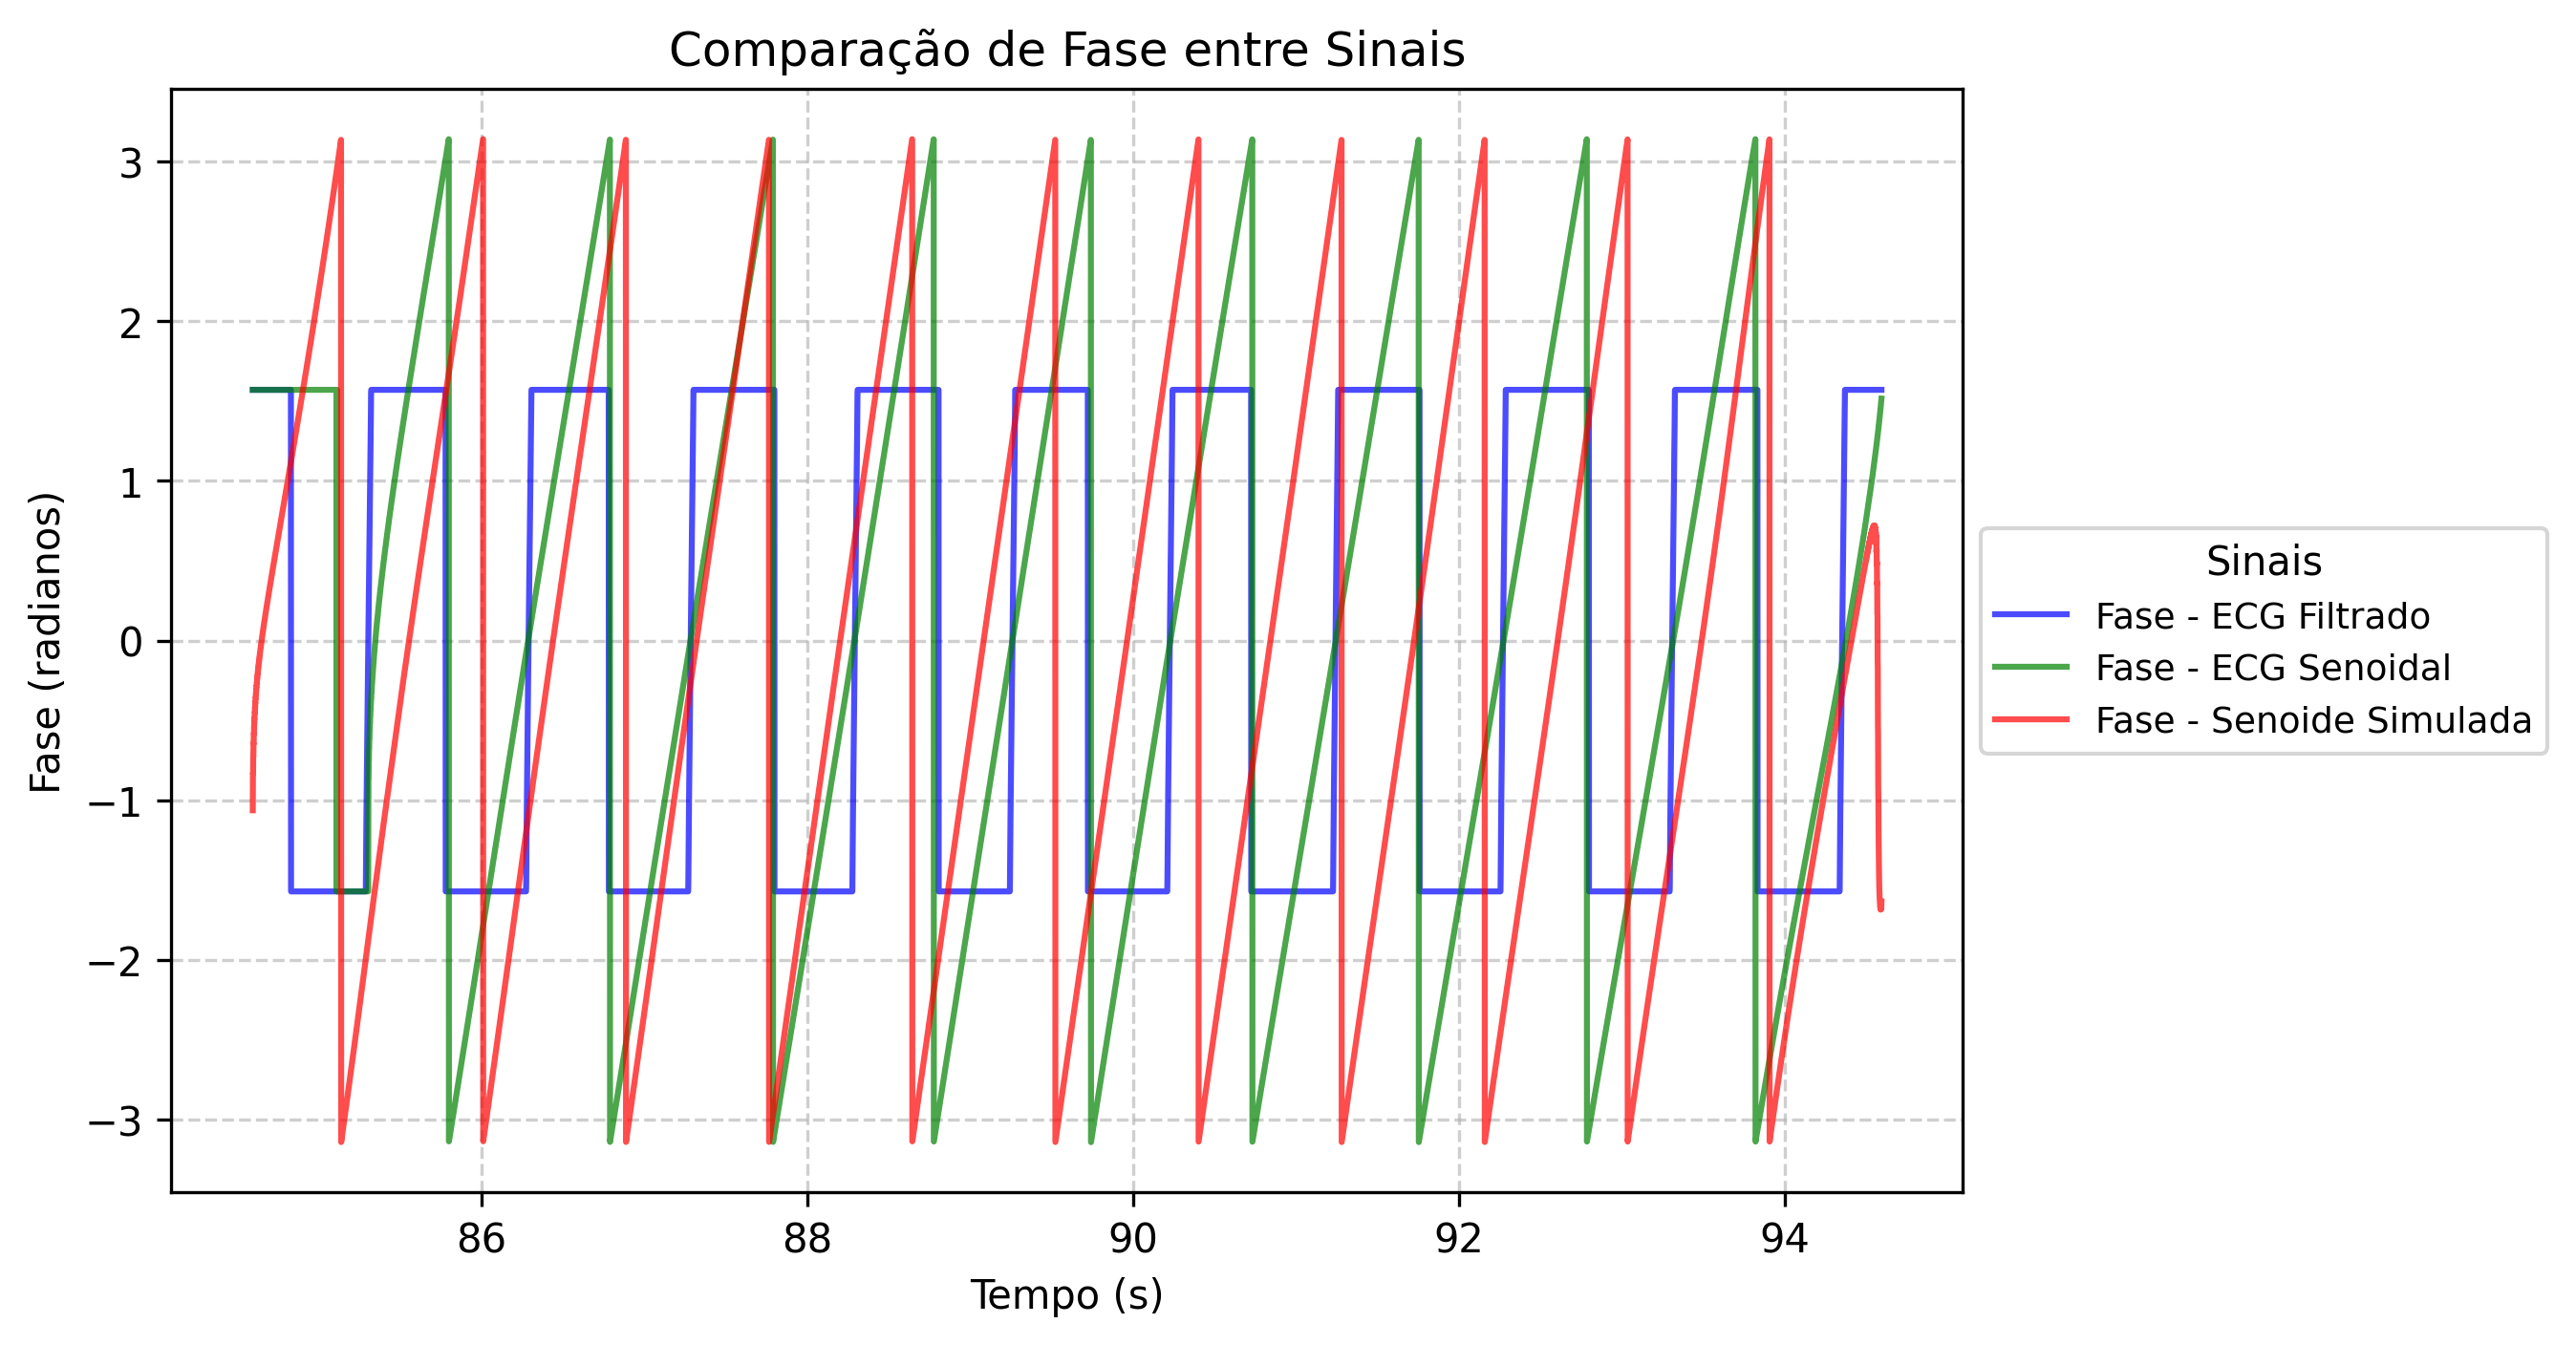
\includegraphics[width=0.8\textwidth]{figs/2_preprocessamento_ecg/3_Comparação_de_Fase_entre_Sinais.png}
    \caption{Exemplo de comparação de fase entre o ECG filtrado (azul), o ECG senoidal (verde) e um sinal simulado (vermelho). A boa concordância entre as fases indica que o procedimento de geração do sinal senoidal e a extração de fase são consistentes.}
    \label{fig:ecg_comparacao_fase}
\end{figure}

Em suma, a transformação do ECG em um sinal senoidal não apenas define de forma clara o ciclo cardíaco, mas também possibilita a extração de uma fase contínua, fundamental para a análise de sincronização de fase entre EEG e ECG utilizando métodos que envolvam extração de fase, tais quais os utilizados neste estudo.

\subsubsection{Estrutura do Dado Final e Armazenamento}

O DataFrame final resultante do processamento do ECG integra:
\begin{itemize}
    \item \textbf{Tempo:} Timestamps sincronizados.
    \item \textbf{Sinal Bruto (EMG):} Valor original do sinal.
    \item \textbf{Sinal Limpo (ECG):} Versão filtrada do sinal.
    \item \textbf{Picos:} Indicador binário dos R-peaks detectados.
    \item \textbf{First Filtered:} Sinal obtido após a aplicação do filtro de janela (±50 ms).
    \item \textbf{Final Filtered:} Sinal final obtido após a combinação dos filtros.
    \item \textbf{ECG Senoidal:} Sinal senoidal derivado dos R-peaks.
\end{itemize}
Este conjunto de dados foi exportado em formato CSV.